\begin{figure}[h]
\centering
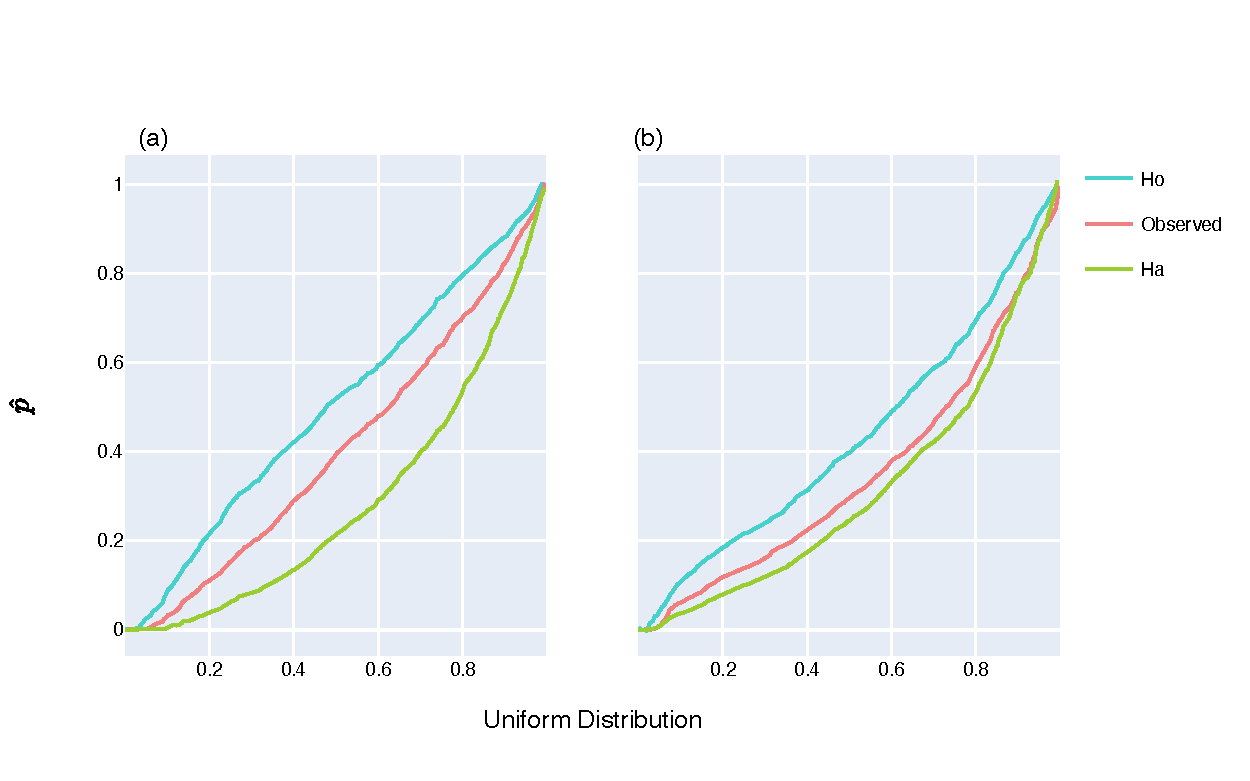
\includegraphics[width=	\textwidth]{figures/plots/primate/LRT-QQ.pdf}
\caption{\textbf{There is a higher proportion of mutation disequilibrium in CDS compared to introns.} The CDS data points appear to fall closer to the positive control than the intronic. The Quantile-Quantile plots compare the distribution of $\hat p-$values to the uniform distribution. \textbf{(a)} 1,406 alignments of introns from human, chimpanzee and gorilla, \textbf{(b)}, 1,182 CDS alignments from human, chimpanzee and gorilla. For all model fitting human was the foreground edge. The observed data points are shown as the pink link, the simulated -ve and +ve controls are shown with the light- and dark-blue lines respectively. }
\label{fig:primate_lrt_qq}
\end{figure}
